\documentclass[11pt,a4paper,twoside]{book}

%\synctex=1

\usepackage{varioref} % intelligent page references
\usepackage{hyperref} % make links

\usepackage{url}
\usepackage{doi} % doi links
%\usepackage{a4wide}
\usepackage[dutch,english]{babel} % use both English and Dutch
\usepackage{amsmath} % all good math stuff
\usepackage{amssymb}
\usepackage[]{graphicx}
\usepackage{float}
\usepackage{subfloat}
\usepackage[hang,bf]{caption} % nice captions and formatting of it
\usepackage{subcaption} 
\usepackage{pdfpages} % insert whole pdf (or pages from it)

\usepackage[toc]{glossaries} % list of abbreviations
\usepackage{imakeidx} % list of abbreviations

\usepackage{rotating} % tables, figures, ... rotated 
\usepackage{arydshln} % advanced package for tables: dashed lines etc
\usepackage[shortcuts]{extdash} % more types of dashes, sometimes useful
\usepackage[version=3]{mhchem} % chemistry symbols: \ce{NH3} gives NH$_3$
\usepackage{booktabs} % Allows the use of \toprule, \midrule and \bottomrule in tables for horizontal lines
\usepackage{cancel} % canceling of terms in math expressions

\usepackage{emptypage} % allows inclusion of empty pdf pages

\usepackage[utf8]{inputenc} % use UTF-8, to make life easier

\usepackage[square,numbers,sort&compress]{natbib}
\usepackage{nicefrac} % nice inline fractions
%\usepackage{subfig} % outdated

\usepackage{algorithm} % nice environment for pseudocode
\usepackage{algpseudocode} % pseudocode

\usepackage{bookmark}
\usepackage{mathrsfs}
\usepackage{xcolor} % colors!
\usepackage{listings} % for source code
\usepackage[nottoc]{tocbibind} % bibliography in ToC but Toc not in ToC
\usepackage[Gray,squaren,thinqspace,thinspace]{SIunits} % Nice way of diplaying numbers and units

\usepackage{braket} % bra ket stuff
\usepackage{csquotes} % nice quotes
\usepackage{amsthm} % for \newtheorem commands
\usepackage[toc,page]{appendix}
\usepackage{mathtools} % for dcases
\usepackage{bbold} 
\usepackage{dsfont} 
\usepackage{chemfig} 
\usepackage{combelow} % Typeset "comma-below" letters, as in Romanian
\usepackage{memhfixc} % for \cleartorecto and \cleartoverso

\usepackage{afterpage} 
% create new blank pages with no style until the next uneven page, not do always work?
\newcommand\blankpage{%
    \null
    \thispagestyle{empty}%
    \addtocounter{page}{-1}%
    \newpage}

\usepackage{epigraph} % for nice quotes in chapters

\usepackage{bibentry} % for list of publications in appendix
%\makeatletter
%\renewcommand\bibentry[1]{\nocite{#1}{\frenchspacing
%     \@nameuse{BR@r@#1\@extra@b@citeb}}}
%\makeatother

% indenting multiline footnotes
\usepackage{scrextend}
\deffootnote{0em}{1.6em}{\thefootnotemark.\enskip}

\usepackage{etoolbox}
% bordermatrix with [ ] instead of ( )
\let\bbordermatrix\bordermatrix
\patchcmd{\bbordermatrix}{8.75}{4.75}{}{}
\patchcmd{\bbordermatrix}{\left(}{\left[}{}{}
\patchcmd{\bbordermatrix}{\right)}{\right]}{}{}

% less white space before subequation
\preto\subequations{\ifhmode\unskip\fi}

% packages not used, but perhaps interesting

%\usepackage{pifont}
%\usepackage{ulem}
%\usepackage{soul}
%\usepackage{makeidx}                    % index
%\usepackage{slantsc}
%\usepackage{placeins}
%\renewcommand*\sfdefault{uop}
%\renewcommand*\familydefault{\sfdefault} 


%% hypersetup
\hypersetup{
    pdfauthor={Ward Poelmans},
    pdftitle={Variational determination of the two-particle density matrix: the case of doubly-occupied space},
 %   pdfkeywords={v2DM, DOCI, Hubbard, GPGPU, cluster},
    pdfsubject={},
%    plainpages=false,
    pdfcreator={\LaTeX\ with package \flqq hyperref\frqq}
    pdfpagelabels,
    bookmarksopen=true,
    bookmarksnumbered=true,
    unicode=true,
}		

%\DeclareUnicodeCharacter{2212}{\textminus}% requires a unicode capable editor
%\usepackage{textcomp}

\newcommand{\minus}{\scalebox{0.75}[1.0]{$-$}} % short minus sign

% papersize required for FEA
\usepackage{geometry}
\geometry{papersize={16cm,24cm},layoutsize={16cm,24cm},top=2cm,bottom=2cm,left=2cm,right=2cm}
\usepackage[strict]{changepage}

% font
\usepackage[T1]{fontenc}
%\usepackage{bera}
\usepackage{libertine}
\renewcommand*\familydefault{\sfdefault}  % biolinum
%\usepackage{libgreek}
%\usepackage[libertine]{newtxmath}

\usepackage{eucal}
%\usepackage{kpfonts}					% ander lettertype
%\usepackage[sc]{mathpazo}
%\linespread{1.05}         % Palatino needs more leading (space between lines)
%\usepackage[T1]{fontenc}

%\usepackage{lmodern} % load a font with all the characters
%\renewcommand*\familydefault{\sfdefault}  % biolinum

%header
\usepackage{fancyhdr}
\pagestyle{fancy}
\widowpenalty=1000
\clubpenalty=1000
\hyphenpenalty=500

\fancyhead[RE]{\slshape \rightmark}
\fancyhead[LO]{\slshape \leftmark}
\fancyhead[RO]{}
\fancyhead[LE]{}

% alinea
\setlength{\parindent}{0pt}
\setlength{\parskip}{1ex plus 0.5ex minus 0.2ex}

\AtBeginEnvironment{adjustwidth}{\partopsep0pt}

% subsubsection: different type of numbering (not 1.11.2 but just roman numbers)
\setcounter{secnumdepth}{3} 	                % use numbers until depth 3
\def\thesubsubsection{\Roman{subsubsection}.}	% romain numbers for index of subsubfigures

% title of chapter
\renewcommand{\chaptermark}[1]{
\markboth{#1}{}
}

% tocdept in table of content
\renewcommand{\sectionmark}[1]{\markright{#1}}
\setcounter{tocdepth}{1}

\setcounter{tocdepth}{3}
\setcounter{secnumdepth}{3}

% custom commands
\newcommand{\pafgeleide}[2]{\frac{\partial #1}{\partial #2}}						% partiele afgeleide
\newcommand{\ptweeafgeleide}[3]{\frac{\partial^2 #1}{\partial #2 \partial #3}}
\newcommand{\afgeleide}[2]{\frac{\mathrm{d} #1}{\mathrm{d} #2}}						% afgeleide
\newcommand{\subsafgeleide}[2]{\frac{\mathrm{D} #1}{\mathrm{D} #2}}					% substantiele afgeleide
\newcommand{\diff}{\mathrm{d}}						 								% rechte d voor dx bvb
\newcommand{\ltransf}{\stackrel{\mathcal{L}}{\longleftrightarrow}}					% pijl laplace
\newcommand{\laplace}{\mathcal{L}}													% teken laplace
\newcommand{\heaviside}{\mathbb{H}}													% Heavisidefunctie
\newcommand{\abs}[1]{\left|#1\right|}												% absolute waarde
\newcommand{\gehelegetallen}{\mathbb{Z}}											% symbool gehele getallen
\newcommand{\complexegetallen}{\mathbb{C}}											% symbool complexe getallen
\newcommand{\verz}[1]{\left\{ #1 \right\}}											% accolades
\newcommand{\vnabla}{\vec{\nabla}}													% Nabla met een vectorteken erboven
\newcommand{\tens}[1]{\boldsymbol{#1}}												% tensorteken
\renewcommand{\vec}[1]{\boldsymbol{#1}}												% vectorteken
\newcommand{\odd}{\mathcal{O}}														% oneven
\newcommand{\even}{\mathcal{E}}														% even
\newcommand{\vet}[1]{\boldsymbol{#1}}												% iets in het vet plaatsen in math omgeving		

\newcommand{\tr}[1]{\mathrm{Tr}\left(#1\right)}
\newcommand{\erdm}[1]{\rho_{#1}}
\newcommand{\trdm}[1]{\Gamma_{#1}}
\newcommand{\drdm}[1]{{^3 \Gamma_{#1}}}

\newcommand{\padd}[1]{\hat{a}_{#1}^{\dagger}}
\newcommand{\pdel}[1]{\hat{a}_{#1}}

\newcommand{\citew}[1]{\citeauthor{#1} \citep{#1}}

%\newcommand{\todo}[1]{}
\newcommand{\todo}[1]{{\color{red}{\textbf{Todo: #1}}}}

\newcommand{\dth}{$\text{D}_\text{2h}$}
\newcommand{\co}{$\text{C}_\text{1}$}
\newcommand{\ctv}{$\text{C}_\text{2v}$}

\newcommand\norm[1]{\left\lVert#1\right\rVert}


%physical properties
\newcommand{\efield}{\mathcal{E}}														% even

% Clebsch-coefficients
\newcommand{\cgc}[6]{ \left\langle #1 \: #2 \; #3 \: #4 \right| #5 \: #6 \left.\right\rangle }

% 3j symbols
\newcommand{\driej}[6]{
    \left(
    \begin{array}{ccc}
        #1 & #3 & #5 \\
        #2 & #4 & #6
    \end{array}
    \right)
}

% reduced matrix element
\newcommand{\rme}[3]{\bigl\langle #1 \bigl|\bigl| #2 \bigr|\bigr| #3 \bigr\rangle}		

\makeatletter
\newcommand{\pushright}[1]{\ifmeasuring@#1\else\omit\hfill$\displaystyle#1$\fi\ignorespaces}
\newcommand{\pushleft}[1]{\ifmeasuring@#1\else\omit$\displaystyle#1$\hfill\fi\ignorespaces}
\newcommand{\specialcell}[1]{\ifmeasuring@#1\else\omit$\displaystyle#1$\ignorespaces\fi}
\makeatother

\graphicspath{{figures/}}

\hyphenation{re-pre-sen-ta-bil-it-y}

\newacronym{1dm}{1DM}{first-order reduced Density Matrix}
\newacronym{2dm}{2DM}{second-order reduced Density Matrix}
\newacronym{3dm}{3DM}{third-order reduced Density Matrix}
\newacronym{ap1rog}{AP1roG}{Antisymmetric Product of one-reference-orbital Geminals}
\newacronym{apg}{APG}{Antisymmetric Product of Geminals}
\newacronym{bpp}{BPP}{Bounded-Error Probabilistic Polynomial Time}
\newacronym{bqp}{BQP}{Bounded-Error Quantum Polynomial Time}
\newacronym{casscf}{CASSCF}{Complete Active Space Self-Consistent Field}
\newacronym{cc}{CC}{Coupled Cluster}
\newacronym{ccd}{CCD}{Coupled Cluster with Double excitations}
\newacronym{cc-pvdz}{cc-pVDZ}{Correlation Consistent Polarized Valence Double Zeta}
\newacronym{ccsdt}{CCSD(T)}{Coupled Cluster with Singles, Doubles and Triples in Perturbation}
\newacronym{ci}{CI}{Configuration Interaction}
\newacronym{cid}{CID}{Configuration Interaction with Double excitations}
\newacronym{cidq}{CIDQ}{Configuration Interaction with Double and Quadruple excitations}
\newacronym{cisd}{CISD}{Configuration Interaction with Single and Double excitations}
\newacronym[description={Edmiston-Ruedeberg localized orbitals}]{er}{ER}{Edmiston-Ruedeberg}
\newacronym[description={Karush–Kuhn–Tucker conditions}]{kkt}{KKT}{Karush–Kuhn–Tucker}
\newacronym{dft}{DFT}{Density Functional Theory}
\newacronym{dmrg}{DMRG}{Density Matrix Renormalization Group}
\newacronym{doci}{DOCI}{Doubly Occupied Configuration Interaction}
\newacronym{flops}{FLOPS}{Floating-Point Operations per Second}
\newacronym{fullci}{FullCI}{Full Configuration Interaction}
\newacronym{fulldoci}{FullDOCI}{Full Doubly Occupied Configuration Interaction}
\newacronym{ghf}{GHF}{General Hartree-Fock}
\newacronym{gvb}{GVB}{General Valence Bond}
\newacronym{hf}{HF}{Hartree-Fock}
\newacronym{ma}{MA}{Merlin-Arthur}
\newacronym{mcscf}{MCSCF}{Multi-Configurational Self-Consistent Field}
\newacronym{mo}{MO}{Molecular Orbital theory}
\newacronym{mpi}{MPI}{Message Passing Interface}
\newacronym{mps}{MPS}{Matrix Product State}
\newacronym{np}{NP}{Nondeterministic Polynomial Time}
\newacronym{p}{P}{Deterministic Polynomial Time}
\newacronym{qma}{QMA}{Quantum Merlin Arthur}
\newacronym{rhf}{RHF}{Restricted Hartree-Fock}
\newacronym{sa}{SA}{Simulated Annealing}
\newacronym{sdp}{SDP}{Semidefinite Programming}
\newacronym{uhf}{UHF}{Unrestricted Hartree-Fock}
\newacronym{v2dm-doci}{v2DM-DOCI}{Variational Optimization of the second-order reduced Density Matrix in the DOCI space}
\newacronym{v2dm}{v2DM}{Variational Optimization of the second-order reduced Density Matrix}
\newacronym{vbscf}{VBSCF}{Valence Bond Self-Consistent Field}
\newacronym{vb}{VB}{Valence Bond}

\newglossaryentry{seniority}
{
  name=seniority,
  description={The number of unpaired particles in the wave function}
}
\newglossaryentry{geminal}
{
  name=geminal,
  description={A two-particle state}
}
\newglossaryentry{size-extensive}
{
  name=size extensive,
  description={The energy scales (linearly) with the number of electrons}
}
\newglossaryentry{size-consistent}
{
  name=size consistent,
  description={The energy of a seperated (dissociated) system is the sum of the energy of its parts}
}

\makeglossaries

\newtheorem{theorem}{Theorem}

% for the papers part, reset chapter numbering a new part
\makeatletter
\@addtoreset{chapter}{part}
\makeatother

% this must be one of the last packages loaded !!
\usepackage{cleveref}

% special links for 'Paper' chapters, try \cref{paper1}
\crefname{mypaper}{Paper}{Papers}

\bibliographystyle{mybibtexstyle} 
%\bibliographystyle{unsrtnat} 
%\nobibliography*

\begin{document}		

\frontmatter

    % front page %
    %%%%%%%%%%%%%%
    \pagenumbering{gobble}

{\large \ \vspace{0.25\textheight} \\

\hspace{-\parindent}Variational determination of the two-particle density matrix: the case of doubly-occupied space\\

\hspace{-\parindent}Variationele bepaling van de tweedeeltjesdichtheidsmatrix in het geval van de dubbel-bezette ruimte


\vspace{0.5cm}
\hspace{-\parindent}Ward Poelmans

}

\vspace*{\fill}
\hspace{-\parindent}Supervisors: prof. dr. D. Van Neck,~ prof. dr. P. Bultinck\\
\hspace{-\parindent}Dissertation submitted in fulfillment of the requirements for the degree of\\
\hspace{-\parindent}Doctor (Ph.D.) in Science: {Physics}\\


\vspace{0.5cm}

\hspace{-\parindent}\begin{minipage}{0.7\textwidth}
  \hspace{-\parindent}Department of Physics and Astronomy\\
%  \hspace{-\parindent}Voorzitter: prof. dr. D. Ryckbosch\\
  \hspace{-\parindent}Faculty of Sciences\\
  \hspace{-\parindent}Ghent University\\
  \hspace{-\parindent}Academic year 2014-2015
\end{minipage}
\begin{minipage}{0.3\textwidth}
  \begin{flushright}
    \includegraphics[width=0.7\textwidth]{./figures/logo-ugent}
  \end{flushright}
\end{minipage}



    % roman numbers for the preamble
    %\includepdf[pages=1-2]{./titelpagina.pdf}
    \pagenumbering{roman}
    \thispagestyle{empty}
%    \setcounter{page}{3}

    \cleardoublepage 
    \thispagestyle{empty}
%    \newpage
    \thispagestyle{empty}

    % CMM page %
    %%%%%%%%%%%%
    \newpage
    \thispagestyle{empty}
    \noindent
    \\
	\vfill
	\begin{figure}[h!]
	  \includegraphics[width=0.15\textwidth]{acknowledge/HPCUGent.jpg} \hspace{0.3cm}
	  \includegraphics[width=0.2\textwidth]{acknowledge/logo_VSC_CMYK2.pdf} \hspace{0.3cm}
	  \includegraphics[width=0.2\textwidth]{acknowledge/hercules.png} \hspace{0.3cm}
	  \includegraphics[width=0.2\textwidth]{acknowledge/EWI.jpg} 
	\end{figure}
	    {\small
	    \noindent \textsf{The computational resources (Stevin Supercomputer Infrastructure) and services used in this work were provided by the VSC (Flemish Supercomputer Center), funded by Ghent University, the Hercules Foundation and the Flemish Government - department EWI.}}
    \vfill
    \begin{figure}[h!]
	    \includegraphics[width=0.6\textwidth]{cmm.png}
    \end{figure}
    {\small
    \noindent \textsf{This research was conducted at the Center for Molecular Modeling.}
    }


    % Quote page %
    %%%%%%%%%%%%%%
%    \cleardoublepage

\vspace*{\fill}
\begin{flushright}
  \textit{You can know the name of a bird in all the languages of the world, but when you're finished, you'll know absolutely nothing whatever about the bird\ldots So let's look at the bird and see what it's doing --- that's what counts.} \\
Richard P. Feynman
\end{flushright}


%    \newpage % strikt noodzakelijk om een header op deze blz. te vermijden

    % Jury page %
    %%%%%%%%%%%%%
    \cleardoublepage
\thispagestyle{empty}

\vspace*{\fill}
\Large
Members of the examination committee

\vspace{0.5cm}
\normalsize
\textbf{Chair} \\

prof. dr. Natalie Jachowicz (Universiteit Gent) \\

\textbf{Reading Committee} \\  

prof. dr. Dimitri Van Neck (Universiteit Gent, \textit{promotor}) \\
prof. dr. Paul W. Ayers (McMaster University) \\
dr. Brecht Verstichel (Universiteit Gent) \\

\textbf{Other members}  \\

prof. dr. Patrick Bultinck (Universiteit Gent, \textit{copromotor}) \\
dr. Stijn De Baerdemacker (Universiteit Gent) \\
prof. dr. ir. An Ghysels (Universiteit Gent) \\
prof. dr. ir. Veronique Van Speybroeck (Universiteit Gent) \\

\vspace*{\fill}


    \cleardoublepage

    \cleardoublepage

\selectlanguage{dutch}
\normalsize

\chapter{Dankwoord}
\setlength{\epigraphrule}{0pt}
\setlength{\epigraphwidth}{0.75\textwidth}
\epigraph{\textit{In science, one should use all available resources to solve difficult problems. One of our most powerful resources is the insight of our colleagues.}}{Peter Agre}

Aan iedereen die heeft meegeholpen, bedankt! Aan iedereen die niet heeft meegeholpen, ook bedankt!


\vspace*{\fill}

\begin{flushright}
Ward Poelmans \\
Gent, \today
\end{flushright}

\vspace*{\fill}

\selectlanguage{english}

% vim: spell spelllang=nl syntax=tex tw=140 


    % table of content etc %
    %%%%%%%%%%%%%%%%%%%%%%%%
    % do not show the ToC in the ToC but do show it in the pdf bookmarks
    \cleardoublepage
    \pdfbookmark{\contentsname}{Contents}
    \tableofcontents

    \chapter{Samenvatting}\label{dutch-summary}

\selectlanguage{dutch}
\hyphenation{re-pres-en-teer-baar-heid}

Alle materie is opgebouwd uit atomen. Democritus had dit al in de 5$^\text{de}$ eeuw v.Chr. gepostuleerd, maar hij kon dit natuurlijk
niet bewijzen. De wereld van het atoom bleek echter moeilijk te doorgronden. Pas vanaf de 19$^\text{de}$ eeuw kwam er echt schot in de zaak.
Men ontdekte dat atomen niet ondeelbaar waren en vond het deeltje dat wij tegenwoordig kennen als het elektron. 
In het begin van de 20$^\text{ste}$ eeuw schakelde de ontdekkingstocht een versnelling hoger.

\selectlanguage{english}

% vim: spell spelllang=nl syntax=tex tw=140 

    \chapter{Abstract}
\setlength{\epigraphrule}{0pt}
\setlength{\epigraphwidth}{0.48\textwidth}
\epigraph{\textit{Nothing is as simple as it seems at first.\\Or as hopeless as it seems in the middle.\\Or as finished as it seems in the end.}}{}

The world at the level of the atom is described by the branch of science called quantum mechanics. 
The world of quantum mechanics is very different from our own macroscopic world. It is governed by probabilities and there is a duality
between particles and waves.
Its foundations were built in the first half of the twentieth century by a large group of physicists.
The crown jewel is given by the Schrödinger equation which describes a system of indistinguishable particles, that interact with each other.
However, an equation alone is not enough: the solution is what interests us. This is a problem, because only for the smallest system is the
analytical solution known. For other systems we must resort to numerical techniques. And even then we are plagued by an exponential scaling
of the Hilbert space.


% vim: spell spelllang=en syntax=tex tw=140 


    \glossarystyle{altlist}
    \printglossary[title=List of Abbreviations and Glossary] % toctitle=Terms and abbreviations]

%    \listoffigures
%    \listoftables
	
%    \afterpage{\null\blankpage}


\mainmatter
    \part{Variational determination of the two-particle density matrix: the case of doubly-occupied space}

\chapter{Introduction}\label{ch1}
\setlength{\epigraphrule}{0pt}
\setlength{\epigraphwidth}{0.75\textwidth}
\epigraph{\textit{We must be clear that when it comes to atoms, language can be used only as in poetry. The poet, too, is not nearly so concerned with describing facts as with creating images and establishing mental connections.}}{Niels Bohr}

Richard Feynman, one of the great physicists of the twentieth century, once asked his students:
\begin{displayquote}
If, in some cataclysm, all of scientific knowledge were to be destroyed, and only one sentence passed on to the next generation of creatures, what statement would contain the most information in the fewest words?
\end{displayquote}
It is an interesting question and a wide range of answers is possible but Feynman's own idea is what is of interest here:
\begin{displayquote}
I believe it is the atomic hypothesis that all things are made of atoms - little particles that move around in perpetual motion, attracting each other when they are a little distance apart, but repelling upon being squeezed into one another. In that one sentence, you will see, there is an enormous amount of information about the world, if just a little imagination and thinking are applied.
\end{displayquote}

\todo{add more}


\section{Variational second-order density matrix optimization}\label{ch1-sec2}

An $N$-particle quantum system with pairwise interactions is governed by a Hamiltonian
\begin{equation}
    \hat H = \hat T + \hat V,
    \label{1-eq15}
\end{equation}
where $\hat T$ are the one-body operators and $\hat V$ the two-body operators. We want to find the ground state energy and wave function,
\begin{equation}
    \hat H \Psi(\vet x) = E_0 \Psi(\vet x),
    \label{1-eq16}
\end{equation}

In the second quantization formalism, the Hamiltonian \eqref{1-eq15} can be written as
\begin{equation}
    \hat H = \sum_{\alpha\beta} T_{\alpha\beta} \padd{\alpha}\pdel{\beta} + \frac14 \sum_{\alpha\beta\gamma\delta} V_{\alpha\beta;\gamma\delta}~ \padd{\alpha}\padd{\beta}\pdel{\delta}\pdel{\gamma},
    \label{1-eq13}
\end{equation}
where $T_{\alpha\beta}=\braket{\alpha|\hat T|\beta}$ and $V_{\alpha\beta;\gamma\delta}=\braket{\alpha\beta|\hat V|\gamma\delta}$ are the one- and two-electron integrals. 
In this work, we only consider Hamiltonians which are field-free (e.g. no magnetic field), non-relativistic and real. The wave function is always over the field $\mathbb{R}$. These are the default assumptions in quantum chemistry.
For atoms and molecules, this means that $\hat T$ is the sum of the electronic kinetic energy and the nuclei-electron attraction, whereas $\hat V$ represents the interelectronic Coulomb repulsion. We always work within the Born-Oppenheimer approximation \citep{szabo_modern_1996}: we assume that the wave function can be split in its electronic and nuclear degrees of freedom and we neglect the latter.
The associated Schrödinger equation in its matrix form is
\begin{equation}
    \hat H \ket{\psi} = E_0 \ket{\psi}.
    \label{1-eq14}
\end{equation}
The most simple solution is the mean-field approximation, also known as \gls{hf}, in which $\ket{\psi}$ is given by a single Slater determinant:
\begin{equation}
    \ket{\psi} = \padd{\alpha_1}\padd{\alpha_2}\ldots\padd{\alpha_N}\ket{}~.
    \label{1-eq17}
\end{equation}
A Slater determinant is nothing more than the antisymmetric linear combination of a set of orthogonal single-particle states.
There are $\frac{M!}{N!(M-N)!}$ possible Slater determinants if the dimension of the single-particle basis is $M$ and $N$ the number of particles. They form a complete basis in which we can expand the wave function
\begin{equation}
    \ket{\psi} = \sum_{\alpha_1 \alpha_2 \alpha_3 \ldots \alpha_N} c_{\alpha_1 \alpha_2 \alpha_3 \ldots \alpha_N} ~ \padd{\alpha_1}\padd{\alpha_2}\padd{\alpha_3}\ldots \padd{\alpha_N} \ket{}.
    \label{1-eq18}
\end{equation}
In the \gls{ci} method \citep{helgaker2007molecular}, the wave function is written as a linear combination of a set of Slater determinants. The coefficients are then optimized to find the lowest energy in \cref{1-eq14}. The difficulty in this method lies in picking a suitable set of Slater determinants. 
The best possible solution within the basis set limit is found when all possible Slater determinant are used. This is called \gls{fullci} and coincides with the exact diagonalization of the Hamiltonian matrix. Unfortunately, this is unfeasible for all but the smallest systems. \todo{rework paragraph}



To make further progress in the \gls{v2dm} method, two clear directions exist: (1) the search for new $N$-representability conditions which
are computationally feasible (cheap); and (2) improving the semidefinite program algorithms to exploit the specific structure of \gls{v2dm}. 
On the first path, \citew{qsep} introduced subsystems constraints to fix the problem of fractional charges \citep{helen_1}. \citew{shenvi}
introduced active-space constraints. Stricter bounds on the two-index conditions were derived \citep{dimi,55Johnson_2013a}. Spin symmetry
and point-group symmetry of molecules were exploited \citep{maz_spin}. A stronger three-index condition was derived \citep{maz_T2_prime}.
System-specific constraints were introduced \citep{maz_ham,218Verstichel_2012}. Even excitation energies were calculated
\citep{12Aggelen_2013} using the variationally optimized \gls{2dm}. Additional constraints for non-singlet states were discussed
\citep{128Aggelen_2012}. Linear inequalities for the \gls{2dm} were found \citep{davidson_3,davidson_2,davidson_1}. This list is far from
conclusive and only aims to give a glance of the activity on the $N$-representability front.
Several books and review papers are written about \gls{v2dm} and they provide an excellent overview of the road so far
\citep{coleman_book,rdm_book,mazz_book,braams_book,maz_review,Ayers20131}.

On the semidefinite programming front, several algorithms were tried and customized to \gls{v2dm}
\citep{cpc_proc,maz_prl,primal_dual,mazziotti_large-scale_2011}. The boundary point method \citep{maz_bp} is currently the fastest, but it
is not always stable. In the convex optimization literature, \gls{v2dm} is known under the category 'very large scale': the most common
semidefinite programming problems are much smaller. There exist general purpose solvers \citep{sdpa1} but they are not efficient enough for
our problem size.

 

% vim: spell spelllang=en  tw=140


% reset all acronyms after the introduction
\glsresetall

\chapter{The $N$-representability problem}\label{ch2}

For a given wave function, the \gls{2dm} can be calculated using its definition. However, when given a random symmetric matrix,
is it possible to find a corresponding (ensemble of) wave function which has the given matrix as the \gls{2dm}? This is the essence of the $N$-representability problem.

\section{General \mbox{$N$-representability} theorem}\label{ch2-general-n-rep}
A graphical depiction of this theorem can be found in \Vref{ch2-fig1}. The boundary of the convex set
of $N$-representable $p$th-order reduced density matrices is formed by an infinite number of tangent hyperplanes, where
each hyperplane represents a $p$-particle Hamiltonian and its ground state energy.
\begin{figure}
    \centering
    
\includegraphics[width=\textwidth]{n-representability}
    \caption{Graphical depiction of the necessary and sufficient conditions for $N$-representability. Every Hamiltonian $H^{(p)}$ can be represented by a hyperplane that bounds the convex set of $N$-representable ${^p\Gamma}$.}
    \label{ch2-fig1}
\end{figure}

\section{Approximately $N$-representability conditions}\label{2-approx-n-representability}
In \Vref{ch2-general-n-rep} we showed the necessary and sufficient conditions for $N$-representability. These required the knowledge of the
ground state energy of every possible Hamiltonian and are thus not usable as a sufficient condition. We can, however, use it as a necessary
condition: if we restrict XX to Hamiltonians of which we know the ground state energy or a lower bound on it, we can approximate the convex set of $N$-representable \gls{2dm}'s.
\begin{figure}
    \centering
    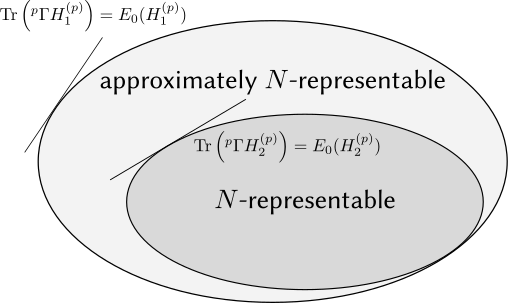
\includegraphics[width=0.9\textwidth]{approx-n-representability}
    \caption{Graphical depiction of the necessary conditions for $N$-representability. $H_1^{(p)}$ belongs to the class of Hamiltonians of which we know a bound on ground state energy while $H_2^{(p)}$ does not. The true convex set of $N$-representable ${^p\Gamma}$ is smaller than the approximate convex set delimited by the Hamiltonians of the class of $H_1^{(p)}$.}
    \label{ch2-fig3}
\end{figure}
In \Vref{ch2-fig3} we give a graphical interpretation of this idea. The approximate set of $N$-representable \gls{2dm} will be larger than the true set: there will be \gls{2dm}'s which fulfil all the necessary conditions but are still not derivable from an ensemble of wave functions.
As a consequence the variational optimization of the \gls{2dm} will give a lower bound on the energy. This is one of the highly attractive features of \gls{v2dm}.

\section{Symmetry considerations}\label{ch2-sym}

\subsection{Spatial point group symmetry}\label{ch2-pointsym}

For example, the $\ce{C2H4}$ molecule shown in \Vref{2-fig4} has $D_{2h}$ symmetry.
\begin{figure}[h]
    \centering
    \chemfig{H-[1]C(-[3]H)=C(-[1]H)(-[:-45]H)}
    \caption{The ethylene molecule has $D_{2h}$ symmetry.}
    \label{2-fig4}
\end{figure}
The main two-fold rotation axis is the connecting axis between the two carbon atoms (the z-axis). The two two-fold rotation axes are the x- and y-axis. The three reflection planes are xy, xz and yz.

As an example, we show the character table and the multiplication table of $C_{2}$ group in \Vref{2-tab1}.
\begin{table}
    \begin{subtable}{.5\linewidth}
        \centering
        \begin{tabular}{c|cc}
            & $E$ & $C_2$ \\
            \hline
            A & 1 & 1 \\
            B & 1 & -1
        \end{tabular}
        \caption{Character table of $C_2$}
        \label{2-tab1a}
    \end{subtable}
    ~
    \begin{subtable}{.5\linewidth}
    \centering
    \begin{tabular}{c|cc}
        & A & B \\
        \hline
        A & A & B \\
        B & B & A 
    \end{tabular}
    \caption{Multiplication table of $C_2$}
    \label{2-tab1b}
    \end{subtable}
    \caption{$C_2$ overview: it has 2 classes of operations. The identity operation and rotations over $180\degree$. The two irreducible representations are $A$ and $B$.}
    \label{2-tab1}
\end{table}
The character table contains the trace of the matrices of the irreducible representations. It it split up into conjugacy classes as the trace is invariant under a similarity transformation. These tables are extremely useful for decomposing a representation in its irreducible parts. The first irreducible representation $A$ is called the trivial representation because all the representation matrices (scalars in this case) are one. Every group has this irreducible representation.

\section{The doubly-occupied Hilbert space}\label{ch2-doci}
In previous sections, we only made general assumptions about the (ensemble of) wave functions from which the \gls{2dm} is derivable. All wave functions should be normalized and antisymmetric. For symmetry, we made assumptions on the quantum numbers of the wave function: it should be a singlet wave function, or the wave function should transform according to a certain irreducible representation.
But we could make other or additional assumptions. If we take a look at the \acrfull{fullci} expansion of the wave function, we see that a Slater determinant is the basic building block
\begin{equation}
    \ket{\Psi} = \sum_\mathbf{k} \sum_\mathbf{s} c_{\mathbf{k};\mathbf{s}} ~ \padd{k_1 s_1}\padd{k_2s_2}\ldots\padd{k_Ns_N}\ket{},
        \label{2-eq106}
\end{equation}

% vim: spell spelllang=en syntax=tex  tw=140


\chapter{Semidefinite Programming}\label{ch3}
\epigraph{\textit{Science is knowledge which we understand so well that we can teach it to a computer; and if we don't fully understand something, it is an art to deal with it.}}{Donald E. Knuth}

The world of convex optimization is a rich and interesting world.


Please read \Vref{paper1}. Or simply \cref{paper1}.


% vim: spell spelllang=en syntax=tex tw=140 


\chapter{Results}\label{ch5}
In the previous chapters, we have introduced the concept of the \acrlong{v2dm}.
In \Cref{ch2}, a necessary set of $N$-representability conditions were derived and in \Cref{ch3} we have shown the computational methods
that can be used to do the actual optimization.
It is time to use this knowledge. First we look into \gls{doci} and explain the motivation for the \gls{doci} $N$-representability conditions derived in \Cref{ch2-doci}.
Next, we explore orbital optimization with the goal to combine it with \gls{v2dm} restricted to \gls{doci}. We then try our method on several
benchmark systems to assess its merits.

\section{Introduction}\label{ch5-doci-intro}

Before we begin the story of the marriage between \gls{doci} and \gls{v2dm}, let us take a step back and consider the origins of
\gls{doci}. First we will introduce some classic concepts of wavefunction-based methods \citep{helgaker2007molecular}.

\begin{figure}
    \captionsetup{justification=centering}
    \begin{subfigure}[b]{0.5\textwidth}
        \includegraphics[width=\textwidth]{BH/orbs-scan-0-1.pdf}
        \caption{Orbitals $1A_1$ and $2A_1$,\\ min $\approx$ -0.027 rad}
        \label{5-fig3-01}
    \end{subfigure}
    \quad
    \begin{subfigure}[b]{0.5\textwidth}
        \includegraphics[width=\textwidth]{BH/orbs-scan-0-2.pdf}
        \caption{Orbitals $1A_1$ and $3A_1$,\\ min $\approx$ -0.011 rad}
        \label{5-fig3-02}
    \end{subfigure}
    \begin{subfigure}[b]{0.5\textwidth}
        \includegraphics[width=\textwidth]{BH/orbs-scan-0-3.pdf}
        \caption{Orbitals $1A_1$ and $4A_1$,\\ min $\approx$ 0.000 rad}
        \label{5-fig3-03}
    \end{subfigure}
    \quad
    \begin{subfigure}[b]{0.5\textwidth}
        \includegraphics[width=\textwidth]{BH/orbs-scan-1-2.pdf}
        \caption{Orbitals $2A_1$ and $3A_1$,\\ min $\approx$ 0.463 rad}
        \label{5-fig3-12}
    \end{subfigure}
    \begin{subfigure}[b]{0.5\textwidth}
        \includegraphics[width=\textwidth]{BH/orbs-scan-1-3.pdf}
        \caption{Orbitals $2A_1$ and $4A_1$,\\ min $\approx$ -0.005 rad}
        \label{5-fig3-13}
    \end{subfigure}
    \quad
    \begin{subfigure}[b]{0.5\textwidth}
        \includegraphics[width=\textwidth]{BH/orbs-scan-2-3.pdf}
        \caption{Orbitals $3A_1$ and $4A_1$,\\ min $\approx$ -0.010 rad}
        \label{5-fig3-23}
    \end{subfigure}
    \captionsetup{justification=raggedright}
    \caption{The red curve has been calculated using XX, while the dashed blue curve uses the same transformed reduced Hamiltonian but an optimized 2DM. The min refers to the minimum of the red curve. The \gls{fullci} energy is \mbox{-24.810 E$_\text{h}$}.}
    \label{5-fig3}
\end{figure}


% vim: syntax=tex spell spelllang=en tw=130 


\chapter{Conclusions}\label{ch6}
\setlength{\epigraphrule}{0pt}
\setlength{\epigraphwidth}{0.75\textwidth}
\epigraph{\textit{The true delight is in the finding out rather than in the knowing.}}{Isaac Asimov}


In this work we have introduced the \acrlong{v2dm} to solve the many-body problem.
The \acrfull{2dm} contains all necessary information to describe such a system, and the expectation value of one- or two-particle operators
can be expressed as a linear function of the \gls{2dm}.
Unlike the more conventional quantum mechanical methods, the wave function is never used. This method itself has a long history and attracted quite some attention in the second half of
the previous century. At first glance, it has many interesting properties: the \gls{2dm} has a much better scaling than the wave function,
and the method is strictly variational. Unlike wavefunction-based methods, it produces a strict lower bound on the energy (instead of an
upper bound).
Unfortunately, the complexity of the many-body problem has not disappeared, but is shifted to the $N$-representability problem: what are the
necessary and sufficient conditions for a \gls{2dm} to be derivable from an ensemble of many-fermion wave functions?
In the 1960's, there was still hope that this problem could be solved in some way, but time has learned that it is a very hard problem (see
later).

% vim: spell spelllang=en syntax=tex tw=140 


%\afterpage{\null\blankpage}

    \part{Papers}
    \let\oldchaptername\chaptername
    \let\oldthechapter\thechapter

%    \renewcommand\thechapter{\Roman{chapter}} % if you want roman numbering
    \renewcommand{\chaptername}{Paper}

    \chapter{Variational Two-Particle Density Matrix Calculation for the Hubbard Model Below Half Filling Using Spin-Adapted Lifting Conditions}
    \label[mypaper]{paper1}
    \includepdf[pages=-]{papers/paper1.pdf}


    % Appropriate credit for the requested material should be given as follows: "Reprinted (adapted) with permission from (COMPLETE REFERENCE CITATION). Copyright (YEAR) American Chemical Society." Insert appropriate information in place of the capitalized words. 


    % APPENDIX &
    %%%%%%%%%%%%

%\afterpage{\null\blankpage}

\bookmarksetupnext{level=part} % puts the bookmark at the same level as a part
\begin{appendices}
    \chapter{List of publications}\label{app-papers}

\begin{itemize}
%\item \bibentry{ward-doci}
%\item \bibentry{mario-doci}
%\item \bibentry{VanHouteghem2014}
%\item \bibentry{deltadftcodes}
    % Verstichel2014, 218Verstichel_2012, 99Verstichel_2013, chemps1, chemps3
  \item B. Verstichel, H. van Aggelen, W. Poelmans, D. Van Neck, 
    \textquote{Variational Two-Particle Density Matrix Calculation for the Hubbard Model Below Half Filling Using Spin-Adapted Lifting Conditions}, 
    \textit{Physical Review Letters} \textbf{108}, 213001 (2012)
  \item B. Verstichel, H. van Aggelen, W. Poelmans, S. Wouters, D. Van Neck, 
    \textquote{Extensive v2DM study of the one-dimensional Hubbard model for large lattice sizes: Exploiting translational invariance and parity}, 
    \textit{Computational and Theoretical Chemistry} \textbf{1003}, 12-21 (2013)
  \item B. Verstichel, W. Poelmans, S. De Baerdemacker, S. Wouters, D. Van Neck, 
      \textquote{Variational optimization of the 2DM: approaching three-index accuracy using extended cluster constraints},
      \textit{The European Physical Journal B} \textbf{87}, 59 (2014)
  \item  S. Wouters, W. Poelmans, P.W. Ayers, D. Van Neck,
      \textquote{CheMPS2: a free open-source spin-adapted implementation of the density matrix renormalization group for ab initio quantum chemistry}, 
      \textit{Computer Physics Communications}, \textbf{185}, 1501-1514 (2014)
  \item M. Van Houteghem, A. Ghysels, T. Verstraelen, W. Poelmans, M. Waroquier, V. Van Speybroeck,
      \textquote{Critical analysis of the accuracy of models predicting or extracting liquid structure information},
      \textit{Journal of Physical Chemistry B}, \textbf{118}, 2451–2470, (2014)
  \item S. Wouters, W. Poelmans, S. De Baerdemacker, P.W. Ayers, D. Van Neck,
      \textquote{CheMPS2: Improved DMRG-SCF routine and correlation functions},
      \textit{Computer Physics Communications}, \textbf{191}, 235-237, (2015)
  \item W. Poelmans, M. Van Raemdonck, B. Verstichel, S. De Baerdemacker, A. Torre, L. Lain, G. Massaccesi, D. Alcoba, P. Bultinck,  D. Van Neck, 
      \textquote{Variational optimization of the second order density matrix corresponding to a seniority-zero configuration interaction wave function},
      \textit{Journal of Chemical Theory and Computation}, \textbf{11}, 4064-4076, (2015) 
  \item M. Van Raemdonck, D. Alcoba,  W. Poelmans, S. De Baerdemacker, A. Torre, L. Lain, G. Massaccesi, P. Bultinck,  D. Van Neck, 
      \textquote{Polynomial scaling approximations and Dynamic Correlation Corrections to Doubly Occupied Configuration Interaction wave functions},
      \textit{Journal of Chemical Physics}, \textbf{143}, 104106  (2015)
  \item K. Lejaeghere, G. Bihlmayer, T. Bj\"orkman, P. Blaha, S. Bl\"ugel, V. Blum, D. Caliste, I. E. Castelli, S. J. Clark, A. Dal Corso, S. de
      Gironcoli, T. Deutsch, J. Kay Dewhurst, I. Di Marco, C. Draxl, M. Du{\l}ak, O. Eriksson, J. A. Flores-Livas, K. F. Garrity, L. Genovese, P.
      Giannozzi, M. Giantomassi, S. Goedecker, X. Gonze, O. Gr{\aa}n\"as, E. K. U. Gross, A. Gulans, F. Gygi, D. R. Hamann, P. J. Hasnip, N. A. W.
      Holzwarth, D. Iu\cb{s}an, D. B. Jochym, F. Jollet, D. Jones, G. Kresse, K. Koepernik, E. K\"u\c{c}\"ukbenli, Y. O. Kvashnin, I. L. M. Locht, S.
      Lubeck, M. Marsman, N. Marzari, U. Nitzsche, L. Nordstr\"om, T. Ozaki, L. Paulatto, C. J. Pickard, W. Poelmans, M. I. J. Probert, K. Refson, M.
      Richter, G. Rignanese, S. Saha, M. Scheffler, M. Schlipf, K. Schwarz, S. Sharma, F. Tavazza, P. Thunstr\"om, A. Tkatchenko, M. Torrent, D.
      Vanderbilt, M. J. van Setten, V. Van Speybroeck, J. M. Wills, J. R. Yates, G. Zhang, S. Cottenier,
      \textquote{The Kohn-Sham equation of state for elemental solids: a solved problem},
      \textit{Science} (2015) (submitted)
\end{itemize}

% vim: syntax=tex spell spelllang=en tw=150


\end{appendices}


\backmatter

    \bookmarksetupnext{level=part} % puts the bookmark at the same level as a part
    \bibliography{refs}

\end{document}

% vim: spell spelllang=en
